\begin{name}
 {Biên soạn: Đỗ Minh Phúc \\ Phản biện: Đoàn Thị Lý}
 {Đề ôn tập chương I}
\end{name}

\caulc
\Opensolutionfile{ans}[ans/ans\currfilebase-Phan-I]
\begin{ex}%[2-D1B5-SO-14-2425]%[VN-MT-7, Đỗ Minh Phúc]%[2D1H1-1]
 Cho hàm số $y=f(x)$ có đạo hàm $f'(x)=-x^2-4$, $\forall x \in \mathbb{R}$. Mệnh đề nào dưới đây đúng?
\choice
{Hàm số đồng biến trên khoảng $(2;+\infty)$}
{Hàm số đồng biến trên khoảng $(-2;2)$}
{\True Hàm số nghịch biến trên khoảng $(-\infty;+\infty)$}
{Hàm số đồng biến trên khoảng $(-\infty;-2)$}
\loigiai{
Do hàm số $y=f(x)$ có đạo hàm $f'(x)=-x^2-4<0$, $\forall x \in \mathbb{R}$ nên hàm số nghịch biến trên khoảng $(-\infty;+\infty)$.
}
\end{ex}

\begin{ex}%[2-D1B5-SO-14-2425]%[VN-MT-7, Đỗ Minh Phúc]%[2D1N2-2]
 Cho hàm số $y=f(x)$ có bảng biến thiên như sau.
 \begin{center}
 
\begin{tikzpicture}
 \tkzTabInit[nocadre,lgt=1.2,espcl=2.5,deltacl=0.6]
 {$x$/0.6,$f'(x)$/0.6,$f(x)$/2}
 {$-\infty$,$-1$,$2$,$+\infty$}
 \tkzTabLine{,+,0,-,0,+,}
 \tkzTabVar{-/$-\infty$,+/$1$,-/$-2$,+/$+\infty$}
 \end{tikzpicture}
 \end{center}
 Giá trị cực tiểu của hàm số đã cho bằng
 \choice
 {$-1$}
 {$2$}
 {\True $-2$}
 {$1$}
\loigiai{
 Dựa vào bảng biến thiên, ta có giá trị cực tiểu của hàm số đã cho bằng $-2$.}
\end{ex}

\begin{ex}%[2-D1B5-SO-14-2425]%[VN-MT-7, Đỗ Minh Phúc]%[2D1N3-2]
 Cho hàm số $y=f(x)$ liên tục trên $\mathbb{R}$ và có bảng biến thiên như sau.
 \begin{center}
 
\begin{tikzpicture}
 \tkzTabInit[nocadre,lgt=1.2,espcl=2.5,deltacl=0.6]
 {$x$/0.6,$y'$/0.6,$y$/2}
 {$-\infty$,$0$,$2$,$+\infty$}
 \tkzTabLine{,+,0,-,0,+,}
 \tkzTabVar{-/$2$,+/$4$,-/$-5$,+/$2$}
 \end{tikzpicture}
\end{center}
 Tổng giá trị lớn nhất và giá trị nhỏ nhất của hàm số $y=f(x)$ trên $\mathbb{R}$ bằng
 \choice
 {$6$}
 {$9$}
 {$-3$}
 {\True $-1$}
 \loigiai{
 Trên $\mathbb{R}$, ta có giá trị lớn nhất của hàm số $y=f(x)$ bằng $4$ tại $x=0$ và giá trị nhỏ nhất bằng $-5$ tại $x=2$.\\
 Khi đó tổng giá trị lớn nhất và giá trị nhỏ nhất của hàm số $y=f(x)$ trên $\mathbb{R}$ bằng $-1$.
}
\end{ex}

\begin{ex}%[2-D1B5-SO-14-2425]%[VN-MT-7, Đỗ Minh Phúc]%[2D1N3-1]
 \immini[thm]{Cho hàm số $y=f(x)$ có đồ thị như hình vẽ. Giá trị lớn nhất của hàm số trên đoạn $[0;3]$ bằng
 \choice
 {\True $4$}
 {$2$}
 {$3$}
 {$0$}}{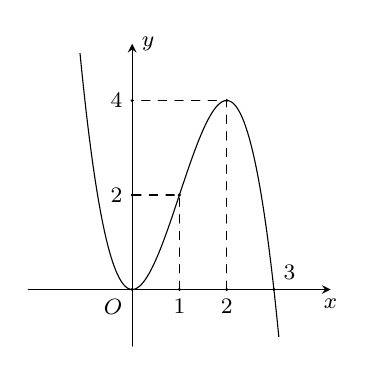
\begin{tikzpicture}[scale=0.6, font=\footnotesize, line join=round, line cap=round, >=stealth]
 \def\xmin{-2}\def\xmax{4}\def\ymin{-1}\def\ymax{5}
 \draw[->] (\xmin-0.2,0)--(\xmax+0.2,0) node[below] {$x$};
 \draw[->] (0,\ymin-0.2)--(0,\ymax+0.2) node[right] {$y$};
 \draw (0,0) node [below left] {$O$};
 \foreach \x in {1,2}
 \fill (\x,0)circle (1pt) node [below] {$\x$};
 \foreach \x in {3}
 \fill (\x,0)circle (1pt) node [above right] {$\x$};
 \foreach \y in {2,4}
 \fill (0,\y)circle (1pt) node [left] {$\y$};
 \clip (\xmin,\ymin) rectangle (\xmax,\ymax);
 \draw[smooth,samples=200,domain=\xmin:\xmax] plot (\x,{-1*((\x)^3)+3*((\x)^2)+0*(\x)+0});
 \draw[dashed] (1,0)--(1,2)--(0,2);\fill (1,2) circle (1pt);
 \draw[dashed] (0,0)--(0,0)--(0,0);\fill (0,0) circle (1pt);
 \draw[dashed] (2,0)--(2,4)--(0,4);\fill (2,4) circle (1pt);
\end{tikzpicture}}
 \loigiai{
 Từ đồ thị hàm số $f(x)$ ta có $\max_{[0;3]}f(x)=4$ tại $x=2$.
 }
\end{ex}

\begin{ex}%[2-D1B5-SO-14-2425]%[VN-MT-7, Đỗ Minh Phúc]%[2D1H4-1]
 Đường tiệm cận ngang của đồ thi hàm số $y=\dfrac{2024x+2025}{x-5}$ là
 \choice
 {$y=2025$}
 {\True $y=2024$}
 {$y=1$}
 {$y=-5$}
 \loigiai{
 Ta có $\lim\limits_{x \to +\infty} \dfrac{2024x+2025}{x-5}=2024$ và $\lim\limits_{x \to-\infty} \dfrac{2024x+2025}{x-5}=2024$ nên đồ thị hàm số có đường tiệm cận ngang là $y=2024$. 
 }
\end{ex}

\begin{ex}%[2-D1B5-SO-14-2425]%[VN-MT-7, Đỗ Minh Phúc]%[2D1N4-1]
 Đường tiệm cận đứng của đồ thị hàm số $y=\dfrac{15x-6}{10x+5}$ là
 \choice
 {$x=\dfrac{3}{2}$}
 {$x=-\dfrac{6}{5}$}
 {\True $x=-\dfrac{1}{2}$}
 {$x=\dfrac{2}{5}$}
 \loigiai{
 Điều kiện xác định $x \neq-\dfrac{1}{2}$.\\
 Ta có $\lim\limits_{x \to\left(-\tfrac{1}{2}\right)^+} \dfrac{15x-6}{10x+5}=-\infty$ và $\lim\limits_{x \to\left(-\tfrac{1}{2}\right)^-} \dfrac{15x-6}{10x+5}=+\infty$ nên đồ thị hàm số có đường tiệm cận đứng là $x=-\dfrac{1}{2}$. 
 }
\end{ex}

\begin{ex}%[2-D1B5-SO-14-2425]%[VN-MT-7, Đỗ Minh Phúc]%[2D1H4-1]
 Tiệm cận xiên của đồ thị hàm số $y=\dfrac{-x^2-3x+4}{x}$ là đường thẳng có phương trình nào sau đây?
 \choice
 {\True $y=-x-1$}
 {$y=x-1$}
 {$y=-x+1$}
 {$y=x+1$}
 \loigiai{
 Ta có $a=\lim\limits_{x \to+\infty}\left(\dfrac{-x^2-3x+4}{x+2}:x\right)=\lim\limits_{x \to+\infty} \dfrac{-x^2-3x+4}{x^2+2x}=-1$.\\
 Lại có $b=\lim\limits_{x \to+\infty}\left[\dfrac{-x^2-3x+4}{x+2}-(-1)x\right]=\lim\limits_{x \to+\infty} \dfrac{-x+4}{x+2}=-1$.\\
 (Tương tự, $\lim\limits_{x \to-\infty}\left(\dfrac{-x^2-3x+4}{x+2}:x\right)=-1$, $\lim\limits_{x \to-\infty}\left[\dfrac{-x^2-3x+4}{x+2}-(-1)x\right]=-1$).\\
 Tiệm cận xiên của đồ thị hàm số $y=\dfrac{-x^2-3x+4}{x+2}$ là đường thẳng có phương trình $y=-x-1$.
 }
\end{ex}

\begin{ex}%[2-D1B5-SO-14-2425]%[VN-MT-7, Đỗ Minh Phúc]%[2D1H5-1]
 \immini[thm]{Đường cong ở hình sau là đồ thi của hàm số nào?
 \choice
 {\True $y=-x^3+3x^2-4$}
 {$y=x^3-4$}
 {$y=x^2-4$}
 {$y=-x^2-4$}}{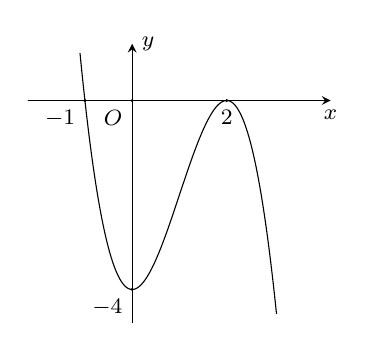
\begin{tikzpicture}[scale=0.6, font=\footnotesize, line join=round, line cap=round, >=stealth]
 \def\xmin{-2}\def\xmax{4}\def\ymin{-4.5}\def\ymax{1}
 \draw[->] (\xmin-0.2,0)--(\xmax+0.2,0) node[below] {$x$};
 \draw[->] (0,\ymin-0.2)--(0,\ymax+0.2) node[right] {$y$};
 \draw (0,0) node [below left] {$O$};
 \foreach \x in {-1}
 \fill (\x,0)circle (1pt) node [below left] {$\x$};
 \foreach \x in {2}
 \fill (\x,0)circle (1pt) node [below] {$\x$};
 \foreach \y in {-4}
 \fill (0,\y)circle (1pt) node [below left] {$\y$};
 \clip (\xmin,\ymin) rectangle (\xmax,\ymax);
 \draw[smooth,samples=200,domain=\xmin:\xmax] plot (\x,{-1*((\x)^3)+3*((\x)^2)+0*(\x)+-4});
 \fill (0,0)circle (1pt);
\end{tikzpicture}}
 \loigiai{
 Xét dáng hình của đồ thị, ta loại được hàm số $y=x^2-4$ và $y=-x^2-4$.\\
 Do $\lim\limits_{x \to+\infty} y=-\infty$ nên ta loại hàm số $y=x^3-4$ và nhận hàm số $y=-x^3+3x^2-4$. 
 }
\end{ex}

\begin{ex}%[2-D1B5-SO-14-2425]%[VN-MT-7, Đỗ Minh Phúc]%[2D1H5-1]
 Hàm số nào sau đây có bảng biến thiên như hình bên dưới?
 \begin{center}
 
\begin{tikzpicture}
 \tkzTabInit[nocadre,lgt=1.2,espcl=2.5,deltacl=0.6]
 {$x$/0.6,$y'$/0.6,$y$/2}
 {$-\infty$,$2$,$+\infty$}
 \tkzTabLine{,-,d,-,}
 \tkzTabVar{+/$2$,-D+/$-\infty$/$+\infty$,-/$2$}
 \end{tikzpicture}
 \end{center}
 \choice
 {\True $y=\dfrac{2x+1}{x-2}$}
 {$y=\dfrac{2x-5}{x-2}$}
 {$y=\dfrac{2x+1}{x+2}$}
 {$y=\dfrac{2x-1}{x+2}$}
 \loigiai{
 Từ bảng biến thiên, ta nhận thấy đồ thị hàm số có tiệm cận đứng là $x=2$ là nên loại hàm số $y=\dfrac{2x+1}{x+2}$ và $y=\dfrac{2x-1}{x+2}$.\\
 Ta nhận thấy hàm số nghịch biến trên từng khoảng xác định nên loại hàm số $y=\dfrac{2x-5}{x-2}$ và nhận hàm số $y=\dfrac{2x+1}{x-2}$.
 }
\end{ex}

\begin{ex}%[2-D1B5-SO-14-2425]%[VN-MT-7, Đỗ Minh Phúc]%[2D1H5-1]
 \immini[thm]{Đường cong ở hình bên là đồ thị của hàm số nào sau đây?
 \choice
 {$y=-x^3+x^2-2x+1$}
 {$y=\dfrac{x^2-x+3}{x-1}$}
 {\True $y=\dfrac{x^2-3x+6}{x-1}$}
 {$y=\dfrac{2x+3}{x-1}$}}{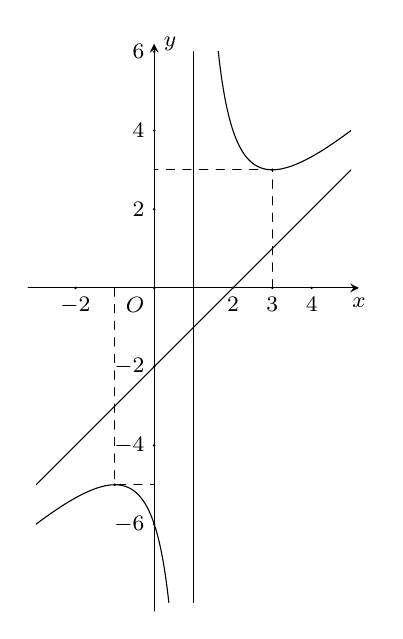
\begin{tikzpicture}[scale=0.5, font=\footnotesize, line join=round, line cap=round, >=stealth]
 \def\xmin{-3}\def\xmax{5}\def\ymin{-8}\def\ymax{6}
 \draw[->] (\xmin-0.2,0)--(\xmax+0.2,0) node[below] {$x$};
 \draw[->] (0,\ymin-0.2)--(0,\ymax+0.2) node[right] {$y$};
 \draw (0,0) node [below left] {$O$};
 \foreach \x in {-2,2,3,4}
 \fill (\x,0)circle (1pt) node [below] {$\x$};
 \foreach \y in {-6,-4,-2,2,4,6}
 \fill (0,\y)circle (1pt) node [left] {$\y$};
 \clip (\xmin,\ymin) rectangle (\xmax,\ymax);
 \draw (1,\ymin)--(1,\ymax);
 \draw[domain=\xmin:\xmax] plot (\x,{1*(\x)+-2});
 \draw[smooth,samples=200,domain=\xmin:0.9] plot (\x,{(1*((\x)^2)+-3*(\x)+6)/(1*(\x)+-1)});
 \draw[smooth,samples=200,domain=1.1:\xmax] plot (\x,{(1*((\x)^2)+-3*(\x)+6)/(1*(\x)+-1)});
 \draw[dashed] (-1,0)--(-1,-5)--(0,-5);\fill (-1,-5) circle (1pt);
 \draw[dashed] (3,0)--(3,3)--(0,3);\fill (3,3) circle (1pt);
 \fill (0,0)circle (1pt);
\end{tikzpicture}}
 \loigiai{
 \begin{itemize}
 \item Xét hàm số $y=-x^3+x^2-2x+1$. Vì đồ thị hàm số $y=-x^3+x^2-2x+1$ không có đường tiệm cận. Suy ra phương án $y=-x^3+x^2-2x+1$ sai.
 \item Xét hàm số $y=\dfrac{x^2-x+3}{x-1}=x+\dfrac{3}{x-1}$.\\
 Ta có
 $\lim\limits_{x \to+\infty}[y-x]=\lim\limits_{x \to+\infty} \dfrac{3}{x-1}=0$ và $\lim\limits_{x \to-\infty}[y-x]=\lim\limits_{x \to-\infty} \dfrac{3}{x-1}=0$.\\
 Do đó đường thẳng $y=x$ là đường tiệm cận xiên của đồ thị hàm số. Suy ra phương án $y=\dfrac{x^2-x+3}{x-1}$ sai.
 \item Xét hàm số $y=\dfrac{x^2-3x+6}{x-1}=x-2+\dfrac{4}{x-1}$.\\
 Ta có $\lim\limits_{x \to 1^-} y=-\infty$ và $\lim\limits_{x \to 1^+} y=+\infty$.\\
 Do đó đường thẳng $x=1$ là đường tiệm cận đứng của đồ thị hàm số.\\
 Lại có $\lim\limits_{x \to+\infty}[y-(x-2)]=\lim\limits_{x \to+\infty} \dfrac{4}{x-1}=0$ và $\lim\limits_{x \to-\infty}[y-(x-2)]=\lim\limits_{x \to-\infty} \dfrac{4}{x-1}=0$.\\
 Do đó đường thẳng $y=x-2$ là đường tiệm cận xiên của đồ thị hàm số.\\
 Hơn nữa, đồ thị hàm số cắt trục tung tại điểm có tung độ bằng $-6$ nên suy ra phương án $y=\dfrac{x^2-3x+6}{x-1}$ đúng.
 \item Xét hàm số $y=\dfrac{2x+3}{x-1}$. Vì đồ thị hàm số $y=\dfrac{2x+3}{x-1}$ không có đường tiệm cận xiên nên phương án $y=\dfrac{2x+3}{x-1}$ sai.
 \end{itemize}
 }
\end{ex}

\begin{ex}%[2-D1B5-SO-14-2425]%[VN-MT-7, Đỗ Minh Phúc]%[2D1V3-6]
 Khi nuôi cá thí nghiệm trong hồ, một nhà khoa học đã nhận thấy rằng: nếu trên mỗi đơn vị diện tích của mặt hồ có $n$ con cá thì trung bình mỗi con cá sau một vụ cân nặng là $P(n)=800-20n$ (g). Hỏi phải thả bao nhiêu con cá trên một đơn vị diện tích của mặt hồ để sau một vụ thu hoạch được nhiều cá nhất?
 \choice
 {$19$}
 {\True $20$}
 {$21$}
 {$22$}
 \loigiai{
 Gọi $F(n)$ là hàm cân nặng của $n$ con cá sau vụ thu hoạch trên một đơn vị diện tích.\\
 Ta có $F(n)=(800-20n) \cdot n=800n-20n^2$.\\
 Để sau một vụ thu hoạch được nhiều cá nhất thì cân nặng của $n$ con cá trên một đơn vị điện tích của mặt hồ là lớn nhất.\\
 Bài toán trở thành tìm $n\in \mathbb{N}^*$ sao cho $F(n)$ đạt giá trị lớn nhất.\\
 Ta có $F'(n)=800-40n$.\\
 Cho $F'(n)=0 \Leftrightarrow 800-40n=0 \Leftrightarrow n=20$.\\
 Ta có bảng biến thiên
 \begin{center}
 
\begin{tikzpicture}
 \tkzTabInit[nocadre,lgt=1.2,espcl=2.5,deltacl=0.6]
 {$n$/0.6,$F'(n)$/0.6,$F(n)$/2}{$-\infty$,$20$,$+\infty$}
 \tkzTabLine{,+,0,-,}
 \tkzTabVar{-/$-\infty$,+/$8\,000$,-/$-\infty$}
 \end{tikzpicture}
 \end{center}
 Vậy phải thả $20$ con cá trên một đơn vị diện tích của mặt hồ để sau một vụ thu hoạch được nhiều cá nhất.
 }
\end{ex}

\begin{ex}%[2-D1B5-SO-14-2425]%[VN-MT-7, Đỗ Minh Phúc]%[2D1H2-1]
 Hàm số $f(x)=x^3-3x^2-9x+1$ đạt cực đại tại điểm
 \choice
 {\True $x=-1$}
 {$x=1$}
 {$x=3$}
 {$x=-3$}
 \loigiai{
 Ta có $f'(x)=3x^2-6x-9$.\\
 Cho $f'(x)=0\Leftrightarrow 3x^2-6x-9=0\Leftrightarrow\hoac{&x=-1\\&x=3.}$\\
 Ta có bảng biến thiên
 \begin{center}
 
\begin{tikzpicture}
 \tkzTabInit[nocadre,lgt=1.2,espcl=2.5,deltacl=0.6]
 {$x$/0.6,$y'$/0.6,$y$/2}
 {$-\infty$,$-1$,$3$,$+\infty$}
 \tkzTabLine{,+,0,-,0,+,}
 \tkzTabVar{-/$-\infty$,+/$6$,-/$-26$,+/$+\infty$}
 \end{tikzpicture}
 \end{center}
 Dựa vào bảng biến thiên, ta thấy hàm số đạt cực đại tại $x=-1$. 
 }
\end{ex}
\Closesolutionfile{ans}

\cauds
\Opensolutionfile{ans}[ans/ans\currfilebase-Phan-II]
\begin{ex}%[2-D1B5-SO-14-2425]%[VN-MT-7, Đỗ Minh Phúc]%[2D1H5-3]
 Cho hàm số $y=2x^{3}+x^{2}-\dfrac{1}{2}x-3$ có đồ thị $(C)$.
 \choiceTF
 {\True Hàm số xác định trên $\mathbb{R}$}
 {Hàm số đồng biến trên $(-\infty;+\infty)$}
 {Hàm số không có cực trị}
 {\True Đồ thị hàm số cắt đường thẳng $y=m$ tại $3$ điểm khi và chỉ khi $-\dfrac{329}{108}<m<-\dfrac{11}{4}$}
 \loigiai{
 Ta có $y'=6x^{2}+2x-\dfrac{1}{2}$.\\
 Cho $y'=0 \Leftrightarrow 6x^{2}+2x-\dfrac{1}{2}=0 \Leftrightarrow \hoac{&x=-\dfrac{1}{2}\\&x=\dfrac{1}{6}.}$\\
 Bảng biến thiên
 \begin{center}
 
\begin{tikzpicture}[>=stealth]
 \tkzTabInit[nocadre,lgt=1,espcl=2,deltacl=0.5]{$x$/1,$y'$/.7,$y$/2}
 {$-\infty$,$-\dfrac{1}{2}$,$\dfrac{1}{6}$, $+\infty$}
 \tkzTabLine{,+,$0$,-,$0$,+,}
 \tkzTabVar{-/$-\infty$,+/$-\dfrac{11}{4}$,-/$-\dfrac{329}{108}$,+/$+\infty$}
 \end{tikzpicture}
 \end{center}
 \begin{itemchoice}
 \itemch {\bf Đúng}.\\
 Tập xác định $\mathbb{R}$.
 \itemch {\bf Sai}.
 \begin{itemize}
 \item Hàm số đồng biến trên $\left(-\infty; -\dfrac{1}{2}\right)$ và $\left(\dfrac{1}{6}; +\infty\right)$.
 \item Hàm số nghịch biến trên $ \left(-\dfrac{1}{2}; \dfrac{1}{6}\right)$.
 \end{itemize}
 \itemch {\bf Sai}.\\
 Hàm số đạt cực đại tại $x_{\text{CĐ}}=-\dfrac{1}{2}$, $y_{\text{CĐ}}=-\dfrac{11}{4}$; hàm số đạt cực tiểu tại $x_{\text{CT}}=\dfrac{1}{6}$, $y_{\mathrm{CT}}=-\dfrac{329}{108}$.
 \itemch {\bf Đúng}.\\
 Dựa vào bảng biến thiên, đồ thị hàm số cắt đường thẳng $y=m$ tại $3$ điểm khi và chỉ khi $-\dfrac{329}{108}<m<-\dfrac{11}{4}$.
 \end{itemchoice} 
 }
\end{ex}

\begin{ex}%[2-D1B5-SO-14-2425]%[VN-MT-7, Đỗ Minh Phúc]%[2D1V5-3]
 \immini[thm]{Cho hàm số $y=f(x)$ xác định trên $\mathbb{R}$. Đồ thị hàm số $y=f'(x)$ cắt trục hoành tại $3$ điểm phân biệt $a$, $b$, $c$ ($a<b<c)$ như hình bên.
 \choiceTF
 {Hàm số $y=f(x)$ đồng biến trên $(-\infty;a)$}
 {Hàm số có $2$ điểm cực trị}
 {\True Giá trị cực đại của hàm số là $f(b)$}
 {\True Biết $ f(b) < 0$. Đồ thị hàm số $ y = f (x)$ cắt trục hoành tại hai điểm phân biệt}
 }
 {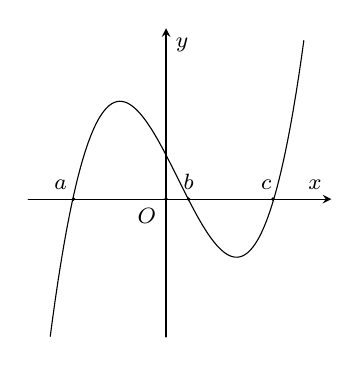
\begin{tikzpicture}[scale=0.7, font=\footnotesize, line join=round, line cap=round, >=stealth]
 \draw[->,black] (-2.5,0) -- (3,0)node[above left] {$x$};
 \draw[->,black] (0,-2.5) -- (0,3.1)node[below right] {$y$};
 \node at (-1.62,0) [above left] {$a$};
 \node at (0.41,0) [above] {$b$};
 \node at (1.82,0) [above] {$c$};
 \node at (0,0) [below left] {$O$};
 \draw[smooth,samples=100,domain=-2.1:2.5] plot(\x,{0.6*(\x)^3-0.4*(\x)^2-1.92*(\x)+0.8});
 \fill %vẽ các điểm rỗng ruột
 (-1.68,0) circle (1pt)
 (0.41,0) circle (1pt)
 (1.94,0) circle (1pt)
 (0,0) circle (1pt);
 \end{tikzpicture}}
 \loigiai{
 Ta có $f'(x)=0\Leftrightarrow\hoac{&x=a\\&x=b\\&x=c.} $
 \begin{center}
 
\begin{tikzpicture}
 \tkzTabInit[nocadre,lgt=1.5,espcl=2.5,deltacl=0.6]
 {$x$/1,$y'$/1,$y$/2}
 {$-\infty$,$a$,$b$,$c$,$+\infty$}
 \tkzTabLine{,-,$0$,+,$0$,-,$0$,+}
 \tkzTabVar{+/ $+\infty$ ,-/$f\left(a\right)$,+/$f\left(b\right)$,-/$f\left(c\right)$,+/ $+\infty$}
 \end{tikzpicture}
 \end{center}
 \begin{itemchoice}
 \itemch {\bf Sai}.\\
 Theo bảng biến thiên, hàm số $y=f(x)$ nghịch biến trên $(-\infty;a)$.
 \itemch {\bf Sai}.\\
 Theo bảng biến thiên, hàm số $y=f(x)$ có $3$ điểm cực trị.
 \itemch {\bf Đúng}.\\
 Theo bảng biến thiên, giá trị cực đại của hàm số là $f(b)$.
 \itemch {\bf Đúng}.\\
 Do $ f(b)<0$ nên đồ thị hàm số cắt trục hoành tại hai điểm phân biệt.
 \end{itemchoice}
 }
\end{ex}

\begin{ex}%%[2-D1B5-SO-14-2425]%[VN-MT-7, Đỗ Minh Phúc]%[2D1H5-4]
 \immini[thm]{Cho hàm số $y=f(x)=\dfrac{ax+b}{cx-1}$ có đồ thị như hình vẽ bên. Các khẳng định sau là đúng hay sai?
 \choiceTF
 {$b=-2$}
 {\True $a+b+c=2$}
 {\True Phương trình $f(x)=1$ có duy nhất một nghiệm}
 {\True Đồ thị hàm số nhận điểm $I(1;-1)$ là tâm đối xứng}
 }
 {\begin{tikzpicture}[scale=0.7,>=stealth, font=\footnotesize, line join=round, line cap=round]
 \def\a{-1} \def\b{2} \def\c{1} \def\d{-1} % Hệ số
 \def\xmin{-3} \def\xmax{5}
 \def\ymin{-4} \def\ymax{4}
 \draw[->] (\xmin,0)--(\xmax,0) node [below]{$x$};
 \draw[->] (0,\ymin)--(0,\ymax) node [left]{$y$};
 \node at (0,0) [above left]{$O$};
 \clip (\xmin+0.1,\ymin+0.1) rectangle (\xmax-0.1,\ymax-0.1);
 \draw[smooth,samples=300,domain=\xmin:(-\d/\c-0.1)] plot(\x,{(\a*(\x)+\b)/(\c*(\x)+\d)});
 \draw[smooth,samples=300,domain=(-\d/\c+0.1:\xmax)] plot(\x,{(\a*(\x)+\b)/(\c*(\x)+\d)});
 \draw (-\d/\c,\ymin)--(-\d/\c,\ymax);
 \draw (\xmin,\a/\c)--(\xmax,\a/\c);
 \foreach \d/\g in{1/135,2/60}
 \draw[fill=black](\d,0)circle(1pt)node[shift={(\g:0.35)}]{$\d$};
 \foreach \d/\g in{-2/180,-1/135}
 \draw[fill=black](0,\d)circle(1pt)node[shift={(\g:0.35)}]{$\d$};
 \fill (0,0) circle (1pt);
 \end{tikzpicture}}
 \loigiai{
 \begin{itemchoice}
 \itemch {\bf Sai}.\\
 Vì điểm $(0;-2)$ thuộc đồ thị hàm số $y=f(x)$ nên ta có $\dfrac{b}{-1}=-2\Leftrightarrow b=2$.
 \itemch {\bf Đúng}.\\
 Vì điểm $(0;-2)$ thuộc đồ thị hàm số $y=f(x)$ nên ta có $\dfrac{b}{-1}=-2\Leftrightarrow b=2$.\\
 Đồ thị hàm số $y=f(x)$ có tiệm cận ngang $y=\dfrac{a}{c}$ và tiệm cận đứng $x=\dfrac{1}{c}$, do đó
 \[\heva{&\dfrac{a}{c}=-1\\&\dfrac{1}{c}=1}\Leftrightarrow \heva{&a=-1\\&c=1.}\]
 Vậy $a+b+c=2$.
 \itemch {\bf Đúng}.\\
 Vẽ đường thẳng $y=1$ trên mặt phẳng tọa độ, ta thấy đường thẳng $y=1$ cắt đồ thị hàm số $y=f(x)$ tại duy nhất một điểm.
 \itemch {\bf Đúng}.\\
 Đồ thị hàm số nhận đường thẳng $y=-1$ làm tiệm cận ngang và $x=1$ là tiệm cận đứng, do đó điểm $(1;-1)$ là tâm đối xứng của đồ thị.
 \end{itemchoice}
 }
\end{ex}

\begin{ex}%[2-D1B5-SO-14-2425]%[VN-MT-7, Đỗ Minh Phúc]%[2D1H4-1]
 Cho hàm số $y=f(x)=\dfrac{x^2+mx-1}{x-1}$.
 \choiceTF
 {Hàm số có cực trị khi và chỉ khi $m\geq 0$}
 {\True Tiệm cận xiên của đồ thị hàm số là đường thẳng $y=x+m+1$}
 {Với $m=1$, hàm số nghịch biến trên khoảng $(0;2)$}
 {Tổng các giá trị nguyên dương của tham số $m$ để hàm số đồng biến trên khoảng $(3;5)$ bằng $6$}
 \loigiai{\begin{itemchoice}
 \itemch {\bf Sai}.\\
 Có $y'=\dfrac{x^2-2x-m+1}{(x-1)^2}$.\\
 Hàm số có hai cực trị khi và chỉ khi phương trình $x^2-2x-m+1=0 $ có hai nghiệm phân biệt khác $1\Leftrightarrow \heva{&\Delta' >0\\&1^2-2\cdot 1-m+1\ne 0} \Leftrightarrow \heva{&m>0\\&m \ne 0} \Leftrightarrow m>0$. 
 \itemch {\bf Đúng}.\\
 Ta có $y=x+m+1+\dfrac{m}{x-1}$.\\
 $\lim\limits_{x\to \pm \infty}\left[y-(x+m+1)\right]=\lim\limits_{x\to\pm \infty}\dfrac{m}{x-1}=0$.\\
 Vậy đồ thị hàm số có tiệm cận xiên $y=x+m+1$.
 \itemch {\bf Sai}.\\
 Với $m=1$, hàm số trở thành $y=\dfrac{x^2+x-1}{x-1}$ không xác định trên khoảng $(0;2)$ nên không nghịch biến trên khoảng $(0;2)$.
 \itemch {\bf Sai}.\\
 Hàm số đồng biến trên khoảng $(3;5)$
 \begin{eqnarray*}
 \Leftrightarrow x^2-2x-m+1\geq 0,\ \forall x\in (3;5)
 &\Leftrightarrow& m\leq x^2-2x+1,\ \forall x\in (3;5)\\
 &\Leftrightarrow& m\leq \min\limits_{[3;5]} \left(x^2-2x+1\right).
 \end{eqnarray*}
 Xét hàm $g(x)=x^2-2x+1 $ có bảng biến thiên
 \begin{center}
 
\begin{tikzpicture}
 \tkzTabInit[nocadre,lgt=1.2,espcl=2.5,deltacl=0.6]
 {$x$/.7 ,$g'(x)$/.7,$g(x)$/2}
 {$-\infty$,$1$,$+\infty$}
 \tkzTabLine{,-,0,+,}
 \tkzTabVar{+/,-/$g(1)$,+/ /}
 \end{tikzpicture}
 \end{center}
 Từ bảng biến thiên suy ra $m\leq g(3) \Leftrightarrow m\leq 4$.\\
 Vì $m$ nguyên dương nên $m \in \{1;2;3;4\}$.\\
 Vậy tổng các giá trị $m$ thỏa mãn yêu cầu đề bài bằng $10$.
 \end{itemchoice}}
\end{ex}
\Closesolutionfile{ans}

\caukq
\Opensolutionfile{ans}[ans/ans\currfilebase-Phan-III]
\begin{ex}%[2-D1B5-SO-14-2425]%[VN-MT-7, Đỗ Minh Phúc]%[2D1V1-3]
 Có bao nhiêu giá trị nguyên của tham số $m$ để hàm số $y=(m-1)x^3-(m-1)x^2+3x+2024$ đồng biến trên tập xác định?
\shortans{10}
\loigiai{
Tập xác định $\mathscr{D}=\mathbb{R}$.\\
Ta có $y'=3(m-1)x^2-2(m-1)x+3$.\\
Hàm số đồng biến trên $\mathbb{R}$ khi $y' \geq 0$, $\forall x \in \mathbb{R} \Leftrightarrow 3(m-1)x^2-2(m-1)x+3 \geq 0$, $\forall x \in \mathbb{R}$.
\begin{itemize}
 \item Nếu $m-1=0 \Leftrightarrow m=1$. Khi đó $y' \geq 0 \Leftrightarrow 3 \geq 0$ luôn đúng $\forall x \in \mathbb{R}$.\\
 Suy ra $m=1$ thoả mãn yêu cầu bài toán.
 \item Nếu $m-1 \neq 0 \Leftrightarrow m \neq 1$.\\
 Khi đó 
 \begin{eqnarray*}
 3(m-1) x^2-2(m-1) x+3 \geq 0, \forall x \in \mathbb{R}
 &\Leftrightarrow&\heva{&\Delta'=(m-1)^2-9(m-1) \leq 0 \\ &a=m-1>0}\\
 &\Leftrightarrow&\heva{&1 \leq m \leq 10 \\ &m>1} \Leftrightarrow 1<m \leq 10\text{ (thỏa mãn)}.
 \end{eqnarray*}
 Mà $m \in \mathbb{Z} \Rightarrow m \in\{2;3;4;5;6;7;8;9;10\}$.
\end{itemize}
Vậy có tất cả $10$ giá trị nguyên của tham số $m$ thoả mãn yêu cầu bài toán.
}
\end{ex}

\begin{ex}%[2-D1B5-SO-14-2425]%[VN-MT-7, Đỗ Minh Phúc]%[2D1V1-3]
 Cho hàm số $y=f(x)$ liên tục trên $\mathbb{R}$ thoả mãn $f'(x)=x(x-1)^2(x-2)^3$. Hàm số $g(x)=f\left(x^2-2x+2\right)$ có bao nhiêu điểm cực trị?
 \shortans{3}
 \loigiai{
 Ta có $f'(x)=0 \Leftrightarrow\hoac{&x=0\\&x=1\\&x=2.}$\\
 Bảng biến thiên
 \begin{center}
 \begin{center}
 
\begin{tikzpicture}[scale=1, font=\footnotesize, line join=round, line cap=round, >=stealth]
 \tkzTabInit[nocadre,lgt=1.2,espcl=2.5,deltacl=0.6]
 {$x$/.6,$f'(x)$/.6,$f(x)$/2}
 {$-\infty$,$0$,$1$,$2$,$+\infty$}
 \tkzTabLine{,+,$0$,-,$0$,-,$0$,+}
 \tkzTabVar{-/$-\infty$,+/$ $,R,-/$ $,+/$+\infty$}
 \end{tikzpicture}
 \end{center}
 \end{center}
 Ta có $g'(x)=(2x-2)f'\left(x^2-2x+2\right)$.\\
 Cho $g'(x)=0 \Leftrightarrow\hoac{&2x-2=0\\&f'\left( x^2-2x+2\right)=0}\Leftrightarrow\hoac{&x=1\\&x^2-2x+2=0\\&x^2-2x+2=1\\&x^2-2x+2=2}\Leftrightarrow\hoac{&x=1\\&x=0\\&x=2.}$\\
 Bảng biến thiên
 \begin{center}
 
\begin{tikzpicture}
 \tkzTabInit[nocadre,lgt=1.2,espcl=2.5,deltacl=0.6]
 {$x$/0.6,$g'(x)$/0.6,$g(x)$/2}
 {$-\infty$,$0$,$1$,$2$,$+\infty$}
 \tkzTabLine{,-,0,+,0,-,0,+,}
 \tkzTabVar{+/$+\infty$,-/,+/,-/,+/$+\infty$}
 \end{tikzpicture}
 \end{center}
 Vây hàm số $g(x)=f\left(x^2-2x+2\right)$ có $3$ điểm cực trị.
 }
\end{ex}

\begin{ex}%[2-D1B5-SO-14-2425]%[VN-MT-7, Đỗ Minh Phúc]%[2D1V3-1]
 Tìm $m$ để giá trị lớn nhất của hàm số $y=\dfrac{x-m}{x+1}$ trên đoạn $[1;3]$ bằng $2$.
 \shortans{-3}
 \loigiai{
 Ta có $y'=\dfrac{1+m}{(x+1)^2}$.
 \begin{itemize}
 \item Trường hợp 1: $1+m>0 \Leftrightarrow m>-1$.\\
 Khi đó $y'>0$, $\forall x \in[1;3]$ nên hàm số $y=\dfrac{x-m}{x+1}$ đồng biến trên đoạn $[1;3]$.\\
 Suy ra $\max _{[1;3]}y=y(3)=\dfrac{3-m}{4}=2 \Leftrightarrow m=-5$ (loại).
 \item Trường hợp 2: $1+m<0 \Leftrightarrow m<-1$.\\
 Khi đó $y'<0$, $\forall x \in[1;3]$ nên hàm số $y=\dfrac{x-m}{x+1}$ nghịch biến trên đoạn $[1;3]$.\\
 Suy ra $\max _{[1;3]}y=y(1)=\dfrac{1-m}{2}=2 \Leftrightarrow m=-3$ (thỏa mãn).
 \end{itemize}
 Vậy $m=-3$ là giá trị cần tìm.
 }
\end{ex}

\begin{ex}%[2-D1B5-SO-14-2425]%[VN-MT-7, Đỗ Minh Phúc]%[2D1V3-6]
 Chị Hà dự định sử dụng hết $4$ m$^2$ kính để làm một bể cá bằng kính có dạng hình hộp chữ nhật không nắp, chiều dài gấp đôi chiều rộng (các mối ghép có kích thước không đáng kể). Bể cá có dung tích lớn nhất bằng bao nhiêu mét khối (kết quả làm tròn đến hàng phần trăm)?
 \shortans{0{,}73}
 \loigiai{
 \begin{center}
 \begin{tikzpicture}[scale=0.8, font=\footnotesize, line join=round, line cap=round, >=stealth]
 \coordinate (B) at (0,0); 
 \coordinate (A) at (2,2);
 \coordinate (C) at (4,0);
 \coordinate (D) at ($(C)-(B)+(A)$);
 \coordinate (B') at ($(B)+(90:3)$);
 \coordinate (C') at ($(C)+(90:3)$);
 \coordinate (D') at ($(D)+(90:3)$);
 \coordinate (A') at ($(A)+(90:3)$);
 \draw (A')--(B')--(C')--(D')--(A') (B)--(B') (C)--(C') (D)--(D')node[right,midway]{$h$} (B)--(C)node[below,midway,sloped]{$2x$}--(D)node[right,midway]{$x$};
 \draw [dashed] (B)--(A)--(D) (A')--(A);
 \end{tikzpicture}
 \end{center}
 Giả sử bể cá có kích thước như hình vẽ, với $x$, $h>0$.\\
 Theo đề bài ta có $2x^2+2xh+4xh=4 \Leftrightarrow h=\dfrac{4-2x^2}{6x}$.\\
 Do $x>0$, $h>0$ nên $4-2x^2>0 \Leftrightarrow 0<x<\sqrt{2}$.\\
 Thể tích của bể cá là $V=2x^2h=\dfrac{4x-2x^3}{3}=f(x)$, với $x \in\left(0;\sqrt{2}\right)$.\\
 Ta có $f'(x)=\dfrac{4}{3}-2x^2$.\\
 Cho $f'(x)=0 \Leftrightarrow \dfrac{4}{3}-2x^2=0\Leftrightarrow x=\dfrac{\sqrt{6}}{3}$ (vì $x>0$).\\
 Bảng biến thiên
 \begin{center}
 
\begin{tikzpicture}
 \tkzTabInit[nocadre,lgt=1.2,espcl=2.5,deltacl=0.6]
 {$x$/0.6,$f'(x)$/0.6,$f(x)$/2}{$0$,$\tfrac{\sqrt{6}}{3}$,$\sqrt{2}$}
 \tkzTabLine{,+,0,-,}
 \tkzTabVar{-/$0$,+/$\tfrac{8\sqrt{6}}{27}$,-/$0$}
 \end{tikzpicture}
 \end{center}
 Vậy bể cá có dung tích lớn nhất bằng $\dfrac{8\sqrt{6}}{27} \mathrm{~m}^3 \approx 0{,}73 \mathrm{~m}^3$.
}
\end{ex}

\begin{ex}%[2-D1B5-SO-14-2425]%[VN-MT-7, Đỗ Minh Phúc]%[2D1V4-2]
 Có bao nhiêu giá trị thực của tham số $m$ để đồ thị hàm số $y=\dfrac{x^2-1}{x^2+(2-m)x+2m+1}$ có đúng hai đường tiệm cận?
 \shortans{3}
 \loigiai{
 Ta có $\lim\limits_{x \to \pm \infty} y=\lim\limits_{x \to \pm \infty} \dfrac{x^2-1}{x^2+(2-m) x+2 m+1}=\lim\limits_{x \to \pm \infty} \dfrac{1-\dfrac{1}{x^2}}{1+(2-m) \dfrac{1}{x}+(2 m+1) \dfrac{1}{x^2}}=1$.\\
 Suy ra đồ thị của hàm số đã cho có đường tiệm cận ngang $y=1$, do vậy đồ thị đó có đúng hai đường tiệm cận khi và chỉ khi đồ thị hàm số có đúng một đường tiệm cận đứng
 $\Leftrightarrow$ phương trình $x^2+(2-m) x+2 m+1=0$ (*) có nghiệm kép hoặc có một nghiệm $x=-1$ và một nghiệm khác $1$ hoặc có một nghiệm $x=1$ và một nghiệm khác $-1$.
 \begin{itemize}
 \item Trường hợp 1: Phương trình (*) có nghiệm kép
 \[\Leftrightarrow \Delta=0 \Leftrightarrow(2-m)^2-4(2m+1)=0 \Leftrightarrow m^2-12 m=0 \Leftrightarrow\hoac{&m=0\\&m=12.}\]
 \item Trường hợp 2: Phương trình (*) một có nghiệm $x=1$ và một nghiệm khác $-1$
 \[\Leftrightarrow\heva{&m=-4\\&m \neq 0}\Leftrightarrow m=-4.\]
 \item Trường hợp 3: Phương trình (*) một có nghiệm $x=-1$ và một nghiệm khác $1$ \[\Leftrightarrow\heva{&m=0\\&m\neq-4}\Leftrightarrow m=0.\]
 \end{itemize}
Vậy có $3$ giá trị của $m$ thỏa mãn yêu cầu bài toán là $m=-4$, $m=0$, $m=12$.
}
\end{ex}

\begin{ex}%[2-D1B5-SO-14-2425]%[VN-MT-7, Đỗ Minh Phúc]%[2D1V1-2]
 \immini[thm]{Cho hàm số $f(x)$ liên tục trên $\mathbb{R}$ và có đồ thị hàm số $y=f'(x)$ như hình vẽ bên. Hàm số $y=f(x)-\dfrac{1}{3}x^3+6x$ đồng biến trên khoảng $(a;b)$. Khi đó giá trị của biểu thức $b-a$ bằng bao nhiêu?}{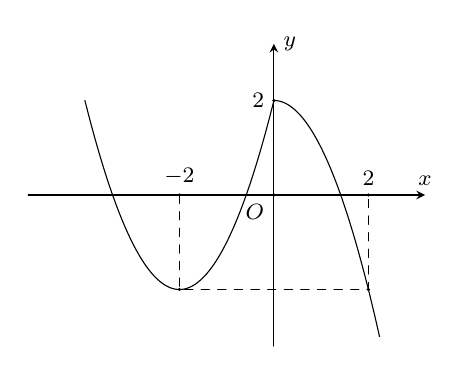
\begin{tikzpicture}[scale=0.6, font=\footnotesize, line join=round,line cap=round,>=stealth]
 \def\xmin{-5}\def\xmax{3}\def\ymin{-3}\def\ymax{3}
 \draw[->] (\xmin-0.2,0)--(\xmax+0.2,0) node[above] {$x$};
 \draw[->] (0,\ymin-0.2)--(0,\ymax+0.2) node[right] {$y$};
 \draw (0,0) node [below left] {$O$};
 \foreach \x in {-2,2}
 \fill (\x,0)circle (1pt) node [above] {$\x$};
 \foreach \y in {2}
 \fill (0,\y)circle (1pt) node [left] {$\y$};
 \clip (\xmin,\ymin) rectangle (\xmax,\ymax);
 \draw[smooth,samples=200,domain=-4:0] plot (\x,{1*((\x)^2)+4*\x+2});
 \draw[smooth,samples=200,domain=0:3] plot (\x,{-1*((\x)^2)+0*\x+2});
 \draw[dashed] (-2,0)--(-2,-2)--(2,-2)--(2,0);
 \fill (-2,-2) circle (1pt);
 \fill (2,-2) circle (1pt);
 \fill (0,0) circle (1pt);
 \end{tikzpicture}}
 \shortans{4}
 \loigiai{
 Ta có $y=f(x)-\dfrac{1}{3} x^3+6 x$ nên $y'=f'(x)-x^2+6$.\\
 Quan sát đồ thị hàm số $y=f'(x)$ và parabol $(P)\colon y=x^2-6$ trên cùng một hệ trục tọa độ như hình vẽ.
 \begin{center}
 \begin{tikzpicture}[scale=0.8, font=\footnotesize, line join=round, line cap=round, >=stealth]
 \def\xmin{-5}\def\xmax{3}\def\ymin{-7}\def\ymax{3}
 \draw[->] (\xmin-0.2,0)--(\xmax+0.2,0) node[above] {$x$};
 \draw[->] (0,\ymin-0.2)--(0,\ymax+0.2) node[right] {$y$};
 \draw (0,0) node [below left] {$O$};
 \foreach \x in {-2,2}
 \fill (\x,0)circle (1pt) node [above] {$\x$};
 \foreach \y in {2}
 \fill (0,\y)circle (1pt) node [left] {$\y$};
 \foreach \y in {-6,-2}
 \fill (0,\y)circle (1pt) node [below right] {$\y$};
 \clip (\xmin,\ymin) rectangle (\xmax,\ymax);
 \draw[smooth,samples=200,domain=-4:0] plot (\x,{1*((\x)^2)+4*\x+2});
 \draw[smooth,samples=200,domain=0:3] plot (\x,{-1*((\x)^2)+0*\x+2});
 \draw[smooth,samples=200,domain=-3:3] plot (\x,{1*((\x)^2)+0*\x+-6});
 \draw[dashed] (-2,0)--(-2,-2)--(2,-2)--(2,0);
 \fill (-2,-2) circle (1pt);
 \fill (2,-2) circle (1pt);
 \fill (0,0) circle (1pt);
 \end{tikzpicture}
 \end{center}
 Từ đồ thị ta có $y'=f'(x)-x^2+6>0 \Leftrightarrow f'(x)>x^2-6 \Leftrightarrow-2<x<2$.\\
 Vậy hàm số $y=f(x)-\dfrac{1}{3}x^3+6x$ đồng biến trên khoảng $(-2;2)$.
}
\end{ex}
\Closesolutionfile{ans}
\begin{indapan}
	{ans/ans\currfilebase}
\end{indapan}

